%
% LaTeX report template 
%

% This is a comment: in LaTeX everything that in a line comes
% after a "%" symbol is treated as comment

\documentclass[11pt, a4paper]{article}
\usepackage{graphicx}
\usepackage{amsmath}
\usepackage{listings}
\usepackage{url}
\usepackage{float}
\usepackage{xcolor}

\definecolor{codegreen}{rgb}{0,0.6,0}
\definecolor{codegray}{rgb}{0.5,0.5,0.5}
\definecolor{codepurple}{rgb}{0.58,0,0.82}
\definecolor{backcolour}{rgb}{0.95,0.95,0.92}

\lstdefinestyle{mystyle}{
    backgroundcolor=\color{backcolour},   
    commentstyle=\color{codegreen},
    keywordstyle=\color{magenta},
    numberstyle=\tiny\color{codegray},
    stringstyle=\color{codepurple},
    basicstyle=\ttfamily\footnotesize,
    breakatwhitespace=false,         
    breaklines=true,                 
    captionpos=b,                    
    keepspaces=true,                 
    numbers=left,                    
    numbersep=5pt,                  
    showspaces=false,                
    showstringspaces=false,
    showtabs=false,                  
    tabsize=2
}

\lstset{style=mystyle}

\title{EE2703: Applied Programming Lab \\ Assignment No 6: The Laplace Transform} % Title

\author{Ishaan Agarwal \\ EE20B046} % Author name

\date{\today} % Date for the report
\begin{document}		
		
\maketitle % Insert the title, author and date

\section{Introduction}
%Create new section;it is autonumbered
The aim of this assignment is to analyse LTI systems using the \texttt{scipy.signal} library.

We majorly use the \texttt{scipy.signal.lsim()} and \texttt{scipy.signal.impulse()} functions to calculate the system response and the inverse Laplace transform respectively.


\section{Questions}
\subsection{Question 1}

We need to solve for the time response of a spring satisfying the equation:
\[\ddot{x} + 2.25x = f(t)\]
where
\[f(t) = \cos(1.5t)\exp(-0.5t)u(t)\]
We solve this by taking Laplace transform on both sides and then taking inverse Laplace of X(s) using \texttt{sp.impulse()} as explained in the code below.

\begin{lstlisting}[language = Python]
#Question 1
#solving an equation using laplace transform

'''given system equation x''+2.25x = f(t)
where f(t) = cos(1.5t)e^(-0.5t)u(t)
and the Laplace transform of f(t) is
F(s) = (s+0.5)/((s+0.5)^2+2.25)

Thus, the given equation in Laplace domain is s^2 X(s) + 2.25 X(s) = F(s)
which implies X(s) = F(s)/(s^2+2.25)
which implies X(s) = (s+0.5) / ( [ (s+0.5)^2 + 2.25 ] [ s^2 + 2.25 ] )
and x(t) = L^-1 (X(s))
'''
#X = (s+0.5) / ( [ s^2 + s + 2.5 ] [ s^2 + 2.25 ] )
X = sp.lti( np.poly1d([1,0.5]) , np.polymul( np.poly1d([1,1,2.5]) , np.poly1d([1,0,2.25]) ) )

#using sp.impulse to calculate the inverse laplace
t,x=sp.impulse(X, None, np.linspace(0,100,1001))

plt.plot(t,x)
plt.xlabel('t')
plt.ylabel('x(t)')
plt.title('x(t) vs t')
plt.show()
\end{lstlisting}

\begin{figure}[H]
     \centering
     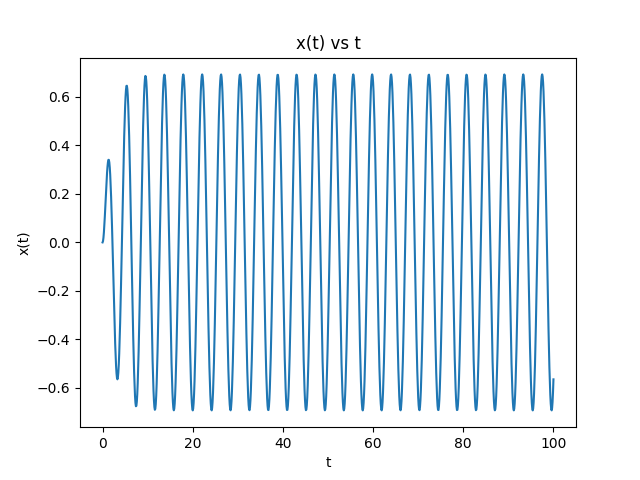
\includegraphics[scale=0.8]{Figure_1.png}
\end{figure}



\subsection{Question 2}

We repeat the same problem with a smaller decay of 0.05 as explained below.

\begin{lstlisting}[language = Python]
#Question 2
#Solving for a much smaller decay of 0.05

'''given system equation x''+2.25x = f(t)
where f(t) = cos(1.5t)e^(-0.05t)u(t)
and the Laplace transform of f(t) is
F(s) = (s+0.5)/((s+0.05)^2+2.25)

Thus, the given equation in Laplace domain is s^2 X(s) + 2.25 X(s) = F(s)
which implies X(s) = F(s)/(s^2+2.25)
which implies X(s) = (s+0.5) / ( [ (s+0.05)^2 + 2.25 ] [ s^2 + 2.25 ] )
and x(t) = L^-1 (X(s))
'''
#X = (s+0.5) / ( [ s^2 + 0.1s + 2.2525 ] [ s^2 + 2.25 ] )
X = sp.lti( np.poly1d([1,0.5]) , np.polymul( np.poly1d([1,0.1,2.2525]) , np.poly1d([1,0,2.25]) ) )

#using sp.impulse to calculate the inverse laplace
t,x=sp.impulse(X, None, np.linspace(0,100,1001))

plt.plot(t,x)
plt.xlabel('t')
plt.ylabel('x(t)')
plt.title('x(t) vs t')
plt.show()
\end{lstlisting}



\begin{figure}[H]
     \centering
     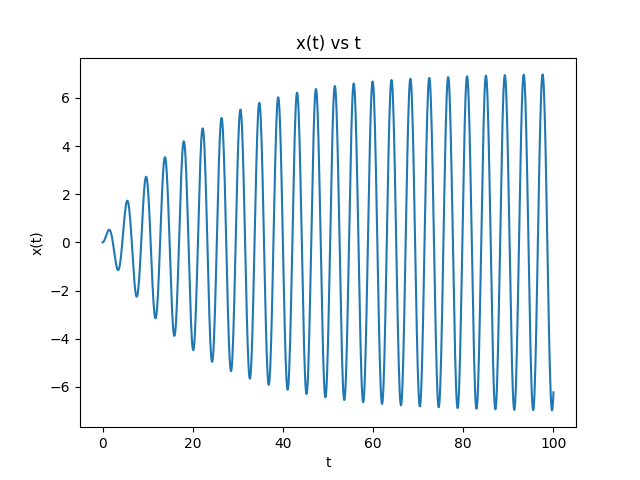
\includegraphics[scale=0.8]{Figure_2.png}
\end{figure}


\subsection{Question 3}
 
This time, we solve the problem for a range of frequencies i.e [1.4, 1.45, 1.5, 1.55, 1.6] by obtaining the transfer $H(s) = X(s)/F(s)$ and then using \texttt{sp.lsim} to calculate the output $x(t)$ for given input signals, as explained in the code below.

\begin{lstlisting}[language = Python]
#Question 3
#Finding the LTI response over a range of frequencies in 1.4 to 1.6 with step of 0.05
for w in np.arange(1.4, 1.6, 0.05):
    H = sp.lti([1], [1, 0, 2.25]) #H(s) = 1/(s^2+2.25)
    t = np.linspace(0, 100, 1000) 
    f = np.cos(w * t) * np.exp(-0.05 * t) #f(t) = cos(wt)e^(-0.05t)u(t)

    #making subplots of the corresponging input and output

    plt.subplot(1, 2, 1)
    plt.plot(t, f)
    plt.xlabel('t')
    plt.ylabel('f(t)')
    plt.title('f(t) vs t for w = ' + str(w))

    t, x, svec = sp.lsim(H, f, t) # using lsim to calculate the output of the system
    plt.subplot(1, 2, 2)
    plt.plot(t, x, 'r')
    plt.xlabel('t')
    plt.ylabel('x(t)')
    plt.title('x(t) vs t for w = ' + str(w))
    plt.show()


\end{lstlisting}



\begin{figure}[H]
     \centering
     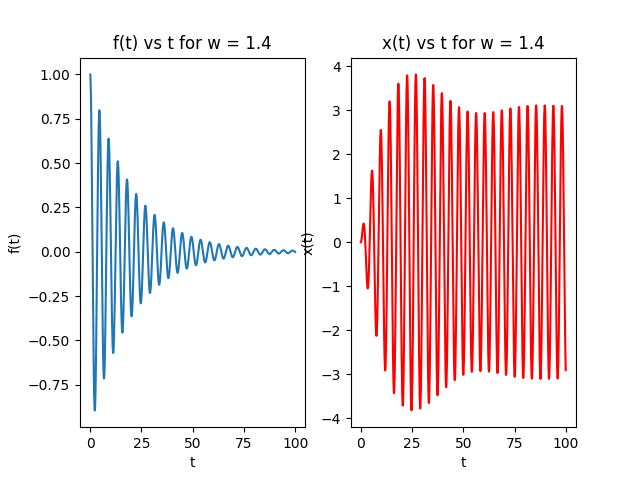
\includegraphics[scale=0.8]{Figure_3.png}
\end{figure}

\begin{figure}[H]
     \centering
     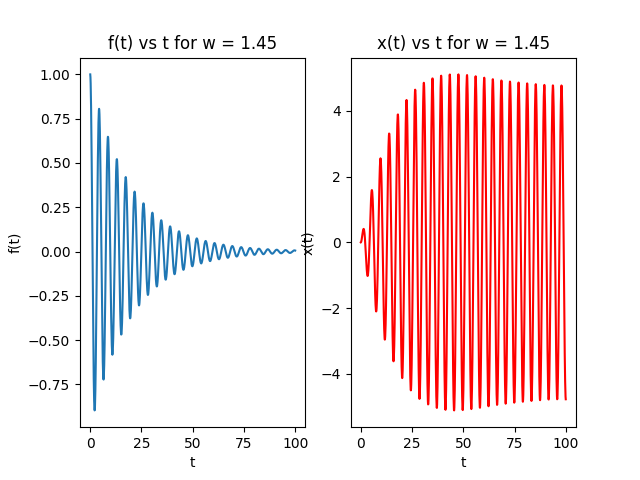
\includegraphics[scale=0.8]{Figure_4.png}
\end{figure}

\begin{figure}[H]
     \centering
     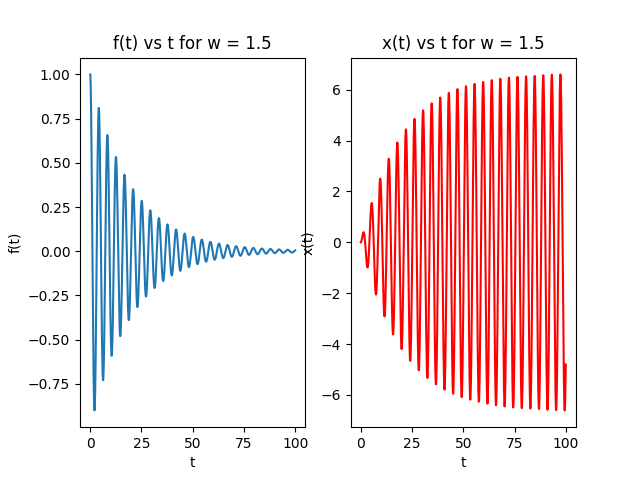
\includegraphics[scale=0.8]{Figure_5.png}
\end{figure}

\begin{figure}[H]
     \centering
     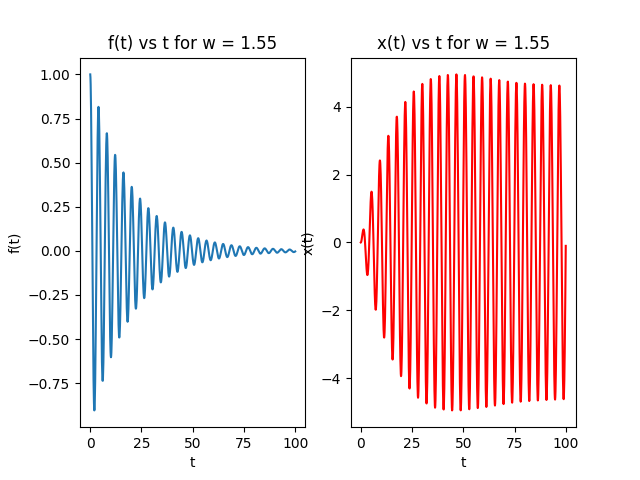
\includegraphics[scale=0.8]{Figure_6.png}
\end{figure}

\begin{figure}[H]
     \centering
     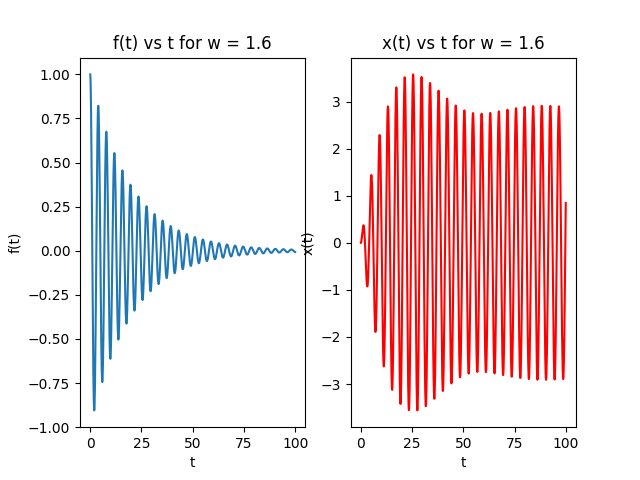
\includegraphics[scale=0.8]{Figure_7.png}
\end{figure}


From the given equation, we notice that the natural frequency of the system is 1.5. We notice that the plot for w = 1.5 has the  highest amplitude, which is understandable from our knowledge of physics, since this is the case of resonance!



\subsection{Question 4}
We have a set of coupled spring equations:
\[\ddot{x} + (x-y) = 0\]
\[\ddot{y} + 2(y-x) = 0\]

On solving these in Laplace domain, with the given initial conditions, we get:
\[X(s) = \frac{s^2+2}{s^3+3s}\]
\[Y(s) = \frac{2}{s^3+3s}\]

Now using inverse Laplace, we obtain $x(t)$ and $y(t)$ and they are plotted in the time interval $0 < t < 20s$ as follows.


\begin{lstlisting}[language = Python]
#Question 4
#Solving for a coupled spring problem
"""
Given Equations:
x'' + x - y =0
y'' + 2y - 2x = 0
subject to initial conditions
x(0) = 1
y(0) = 0
x'(0) = 0
y'(0) = 0
On substituting y from first equation into the second equation, we get
x"" + 3x'' = 0
Taking Laplace Transform keeping initial conditions in mind, this becomes, 
X(s) = (s^2+2) / (s^3 + 3s)
Y(s) = 2/(s^3 + 3s)

"""

t = np.linspace(0, 20, 1001)
X = sp.lti([1, 0, 2], [1, 0, 3, 0])
Y = sp.lti([2], [1, 0, 3, 0])
#using sp.impulse to calculate the inverse laplace
t,x=sp.impulse(X, None, t)
t,y=sp.impulse(Y, None, t)

#plotting x and y
plt.plot(t,x)
plt.plot(t,y)
plt.xlabel('t')
plt.ylabel('x(t) and y(t)')
plt.title('x(t) and y(t) vs t')
plt.legend(['x(t)','y(t)'])
plt.grid()
plt.show()



\end{lstlisting}



\begin{figure}[H]
     \centering
     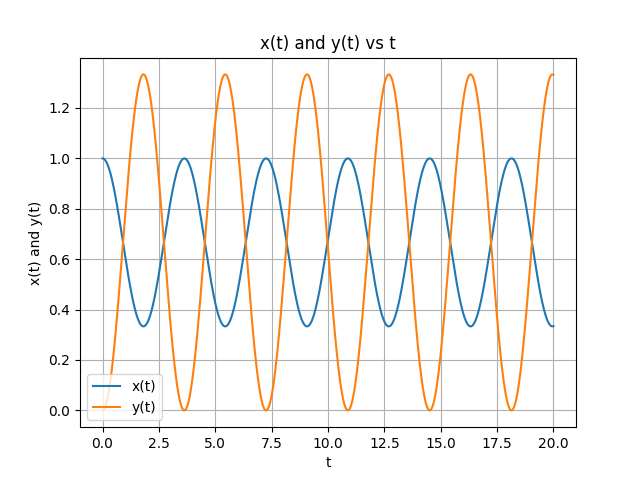
\includegraphics[scale=0.8]{Figure_8.png}
\end{figure}


\subsection{Question 5}

Here, we have an RLC filter with the filter transfer function value as 
\[H(s) = \frac{10^{12}}{s^2+10^8s+10^{12}}\]

We now find and plot the magnitude and phase Bode plots of this filter using \texttt{sp.Bode()} as follows.

\begin{lstlisting}[language = Python]
#Question 5
#To obtain the magnitude and phase of the steady state transfer function of the system
'''
Upon manual solving, we get, 
H(s) = 10^12/( s^2 + 10^8 s + 10^12)
'''
H = sp.lti([10**12], [1, 10**8, 10**12])
#plotting Bode magnitude plot
w, mag, phase = sp.bode(H)
plt.semilogx(w, mag)
plt.xlabel('Frequency')
plt.ylabel('Magnitude')
plt.title('Magnitude Plot of H(s)')
plt.grid()
plt.show()

#plotting Bode phase plot
plt.semilogx(w, phase)
plt.xlabel('Frequency')
plt.ylabel('Phase')
plt.title('Phase Plot of H(s)')
plt.grid()
plt.show()

\end{lstlisting}

\begin{figure}[H]
     \centering
     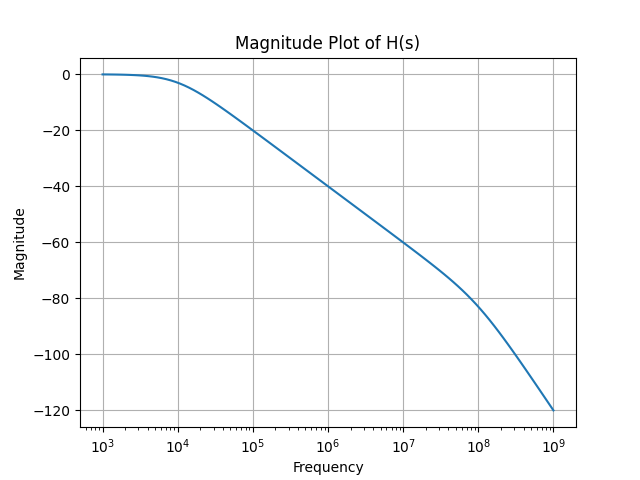
\includegraphics[scale=0.8]{Figure_9.png}
\end{figure}

\begin{figure}[H]
     \centering
     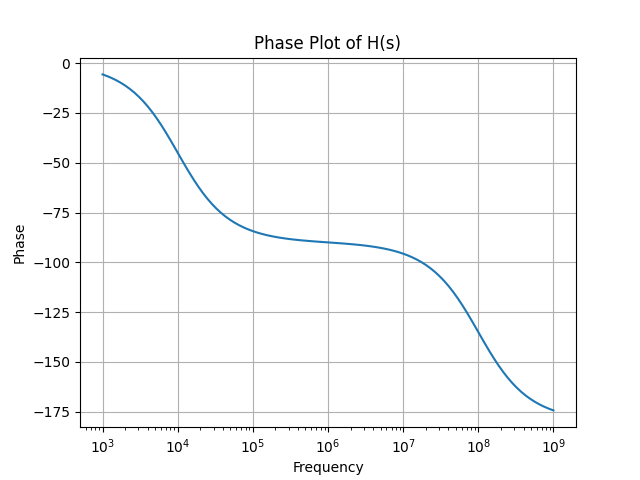
\includegraphics[scale=0.8]{Figure_10.png}
\end{figure}


\subsection{Question 6}

As we have defined our filter in the previous problem, we use that to find the output of our system using \texttt{sp.lsim()}. To capture the fast variation in the beggining, we also solve the problem for the time interval of $0 <t < 30 \mu s$.

\begin{lstlisting}[language = Python]
#Question 6
# vi(t) = cos(10^3t)u(t) - cos(10^6t)u(t)
# To define the transfer function as a system and obtain the output
t1 = np.linspace(0, 0.02, 10001)
t2 = np.linspace(0, 30*10**-6, 10001) #initial time interval zoomed in
vi1 = np.cos(10**3 * t1) - np.cos(10**6 * t1)
vi2 = np.cos(10**3 * t2) - np.cos(10**6 * t2)
H = sp.lti([10**12], [1, 10**8, 10**12])
#Finding the output using sp.lsim
t1, y1, svec = sp.lsim(H, vi1, t1)
t2, y2, svec = sp.lsim(H, vi2, t2)


#plotting the output
plt.plot(t1, y1)
plt.xlabel('t1')
plt.ylabel('y(t)')
plt.title('y(t) vs t')
plt.grid()
plt.show()

plt.plot(t2, y2)
plt.xlabel('t2')
plt.ylabel('y(t)')
plt.title('y(t) vs t')
plt.grid()
plt.show()



\end{lstlisting}

\begin{figure}[H]
     \centering
     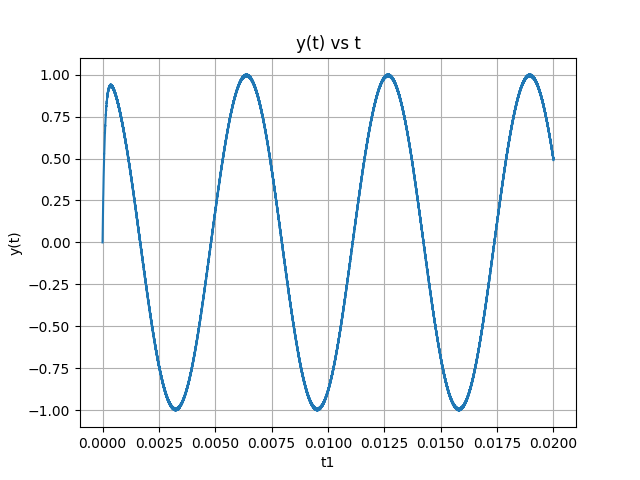
\includegraphics[scale=0.8]{Figure_11.png}
\end{figure}

\begin{figure}[H]
     \centering
     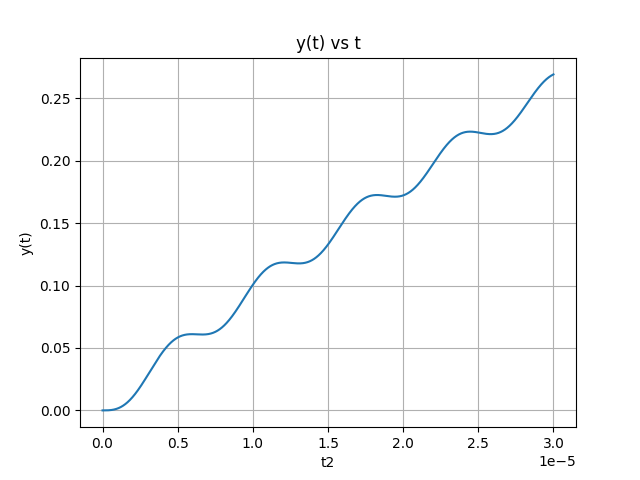
\includegraphics[scale=0.8]{Figure_12.png}
\end{figure}

By manual calculations, we see that the 3-dB bandwidth of the given RLC filter is $10^4$ rad/s. We know that, the signal components with frequency more than the 3-dB bandwidth will be highly attenuated and thus the high frequency component can only be seen as a ripple in the small time interval plot, and is not visible in the large interval time plot. 

\section{Conclusion}
We have learnt to analyse LTI systems using the Laplace tranforms and have learnt to do the same using the \texttt{scipy.signal} library. We have also learnt to calculate time domain response, Bode plots, Laplace tranforms etc. and also plotted graphs for the same. 


\end{document}



 